\documentclass[tikz,border=2pt]{standalone}
\usepackage{amsmath}
\usetikzlibrary{arrows.meta,decorations.pathreplacing}
\begin{document}
% Whole life insurance, one lifetime with T_x = 3.4 (so K_x = 3): immediate settlement pays at T_x,
% PV v^{T_x}; annual settlement pays at the end of the year of death, K_x + 1 = 4, PV v^{K_x+1}.
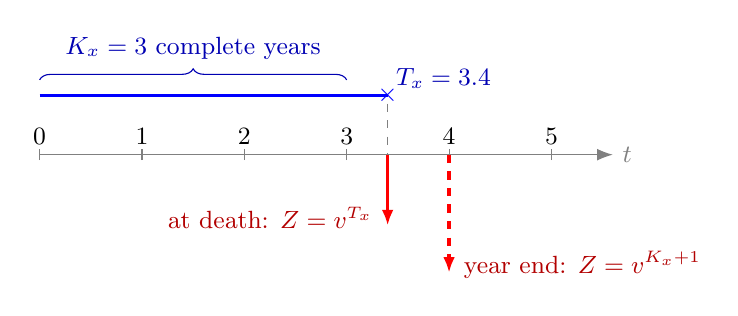
\begin{tikzpicture}[font=\small, >={Latex[length=2mm]}, x=1.3cm]
  \draw[gray, ->] (0,0) -- (5.6,0) node[right] {$t$};
  \foreach \t in {0,...,5} {
    \draw[gray] (\t,-0.07) -- (\t,0.07);
    \node[above, inner sep=2pt] at (\t,0.05) {$\t$};
  }
  % the life
  \draw[blue, very thick] (0,0.75) -- (3.4,0.75);
  \node[blue] at (3.4,0.75) {$\times$};
  \node[blue!70!black, above right, inner sep=1pt] at (3.45,0.8) {$T_x=3.4$};
  \draw[blue!70!black, decorate, decoration={brace, amplitude=4pt}] (0,0.95) -- (3,0.95)
    node[midway, above=4pt] {$K_x=3$ complete years};
  % the two settlement conventions
  \draw[gray, thin, dashed] (3.4,0.65) -- (3.4,0);
  \draw[red, very thick, ->] (3.4,0) -- (3.4,-0.9);
  \node[red!70!black, anchor=east] at (3.35,-0.8) {at death: $Z=v^{T_x}$};
  \draw[red, very thick, dashed, ->] (4,0) -- (4,-1.5);
  \node[red!70!black, anchor=west] at (4.05,-1.4) {year end: $Z=v^{K_x+1}$};
\end{tikzpicture}
\end{document}
